\documentclass[11pt]{article}
\usepackage[margin=1in]{geometry}
\usepackage{graphicx}
\usepackage{booktabs}
\usepackage{xcolor}
\usepackage{hyperref}
\usepackage{float}
\usepackage{amsmath}
\usepackage{caption}
\usepackage{listings}

\hypersetup{colorlinks=true, linkcolor=blue!50!black, citecolor=blue!50!black, urlcolor=blue!50!black}

\title{Week 4: When LSP-Guided Rollback Helps (and When It Doesn't)\\
       \large A Post-Mortem of a Promising Idea That Got Complicated}
\author{CMSC 25750 quarter project}
\date{2026-04-20}

\lstset{basicstyle=\ttfamily\small, breaklines=true, frame=single, xleftmargin=1em, xrightmargin=1em}

\newcommand{\armA}{\textbf{Arm A}}
\newcommand{\armB}{\textbf{Arm B}}

\begin{document}

\maketitle

\begin{abstract}
We evaluate LSP-guided speculative decoding with semantic rollback on the MultiPL-E HumanEval Rust benchmark across 15 open-weight models spanning 0.8B to 123B parameters. The design: generate Rust token-by-token, snapshot at each statement boundary, fire an asynchronous rust-analyzer diagnostic check, and roll back on blocking errors. We compare against a compiler-only retry baseline at matched wall-clock budget. \textbf{The LSP tier almost never fires a blocking classification} — not because the runner is broken, but because the classifier demotion rule needed to avoid forward-reference false positives coincides with precisely the error categories rust-analyzer's native diagnostics emit during partial-code generation. H1 (faster, fewer compiler calls) is falsified. H2 (partial scaling law: bigger models make fewer mistakes but take longer per token) is strongly supported on both arms (Spearman $|\rho|>0.5$, $p<0.05$). H3 (coding-specialized models benefit less from rollback) is confirmed. The negative result points toward a specific architectural next step: replacing native diagnostics with incremental \texttt{cargo check}.
\end{abstract}

\section{Background}
\label{sec:background}

Code-LMs struggle with the Rust borrow checker, lifetimes, and trait bounds: errors that only surface when the full function is submitted to the compiler. Function-level ``generate-then-fix'' retry helps (Week 3 data showed $+12$pp compile rate for Qwen3.5:9B) but is wasteful — the model generates the whole function before learning anything is wrong.

Three prior systems approach this differently:

\begin{itemize}
    \item \textbf{MGD} (Lakhotia et al., NeurIPS 2023) uses rust-analyzer \emph{completions} to constrain token-level generation. No rollback.
    \item \textbf{DSVD} (Guo et al., 2025) trains an internal probe head on the model's own hidden states to trigger rollback. No external verifier.
    \item \textbf{IterGen} (Park et al., ICLR 2025) implements rollback with user-programmed semantic checks. No automatic LSP integration.
\end{itemize}

None combine \emph{external semantic verification} with \emph{statement-boundary rollback} with \emph{error-informed regeneration}. That's the gap this project targets. Week 4's deliverable was a working prototype plus an empirical evaluation against a strong compiler-only baseline.

\subsection{Hypotheses}

\begin{description}
    \item[H1(a) --- Faster.] LSP-guided rollback (\armA) reaches first-pass-compilation in less wall-clock time than compiler-only retry (\armB).
    \item[H1(b) --- Fewer compiler calls.] \armA\ uses fewer \texttt{cargo check} invocations than \armB.
    \item[H2 --- Partial scaling law.] Larger models need fewer compiler calls, but do \emph{not} necessarily save wall-clock due to inference latency scaling with model size.
    \item[H3 --- Coding-specialized ceiling.] Coding-specialized models (\texttt{qwen2.5-coder:32b}, \texttt{devstral-small-2}) benefit less from rollback because first-pass compile rate is already high.
\end{description}

\section{Methods}
\label{sec:methods}

\subsection{The two arms}

Both arms loop under a fixed per-problem wall-clock budget (40\,s for Micro models, 60\,s for $\geq$20B). There is \emph{no} cap on rollback count; wall-clock is the sole termination signal, reflecting real capital cost. History of previous errors stays in the prompt across rollbacks to prevent oscillation.

\textbf{\armA\ --- LSP + compiler}:
\begin{enumerate}
    \item Stream tokens from Ollama; track statement boundaries (\texttt{;} or closing \texttt{\}} at depth 0 in a Rust-aware scanner that handles strings, raw strings, chars, lifetimes, and nested block comments).
    \item At each new boundary, synchronously pull \texttt{textDocument/diagnostic} from rust-analyzer.
    \item Classify returned diagnostics via a three-signal procedure (position, error class, optional temporal stability); errors inside open function bodies that are plausibly forward references are demoted to non-blocking.
    \item On a blocking classification, abort the stream, keep the prefix up to the latest boundary before the earliest error, and re-issue generation with the error message appended to the prompt.
    \item When the function closes cleanly, run \texttt{rustc} and test. On compile failure, add the rustc error to the prompt and restart.
\end{enumerate}

\textbf{\armB\ --- compiler only}: identical loop, minus step 2--4. Just generate, compile, on failure regenerate with error in context.

Ground truth is the compiler; rust-analyzer is a hint. We deliberately did not include an LSP-only arm --- without the compiler check it has no ground truth and is uninterpretable.

\subsection{Models and dataset}

15 open-weight models spanning 0.8B to 123B. Dataset: MultiPL-E HumanEval Rust (156 problems); this run used the first 30 problems for Micro models and the first 20 for larger. Two planned tags (\texttt{gemma4:31b}, \texttt{gemma4:e4b}) failed manifest lookup --- Gemma 4 is not yet in Ollama's library. No LSP-only arm; no problem-count ablation; no random seed variation within a model-arm.

\subsection{Profiler}

Every arm records a per-problem event log across 10 canonical categories (generation, prompt-ingestion, lsp-roundtrip, lsp-wait, cargo-check, classifier, boundary-detect, rollback-overhead, thinking, idle/other). Rollback-overhead captures the Ollama abort-and-re-ingest cost, which is the primary motivation for a Week 5 migration to HuggingFace \texttt{transformers} with \texttt{past\_key\_values} slicing.

\section{Results}
\label{sec:results}

\subsection{Headline metrics}

Figure~\ref{fig:passcompile} shows compile rate and pass@1 versus model size for both arms. Both arms climb rapidly from 0.8B to $\sim$9B, then saturate above 90\% compile / 80\% pass at $\sim$30B and stay there through 120B. The 0.8B and 4B cases show the loudest signal differences between arms; everything above 9B is within a few percentage points.

\begin{figure}[H]
    \centering
    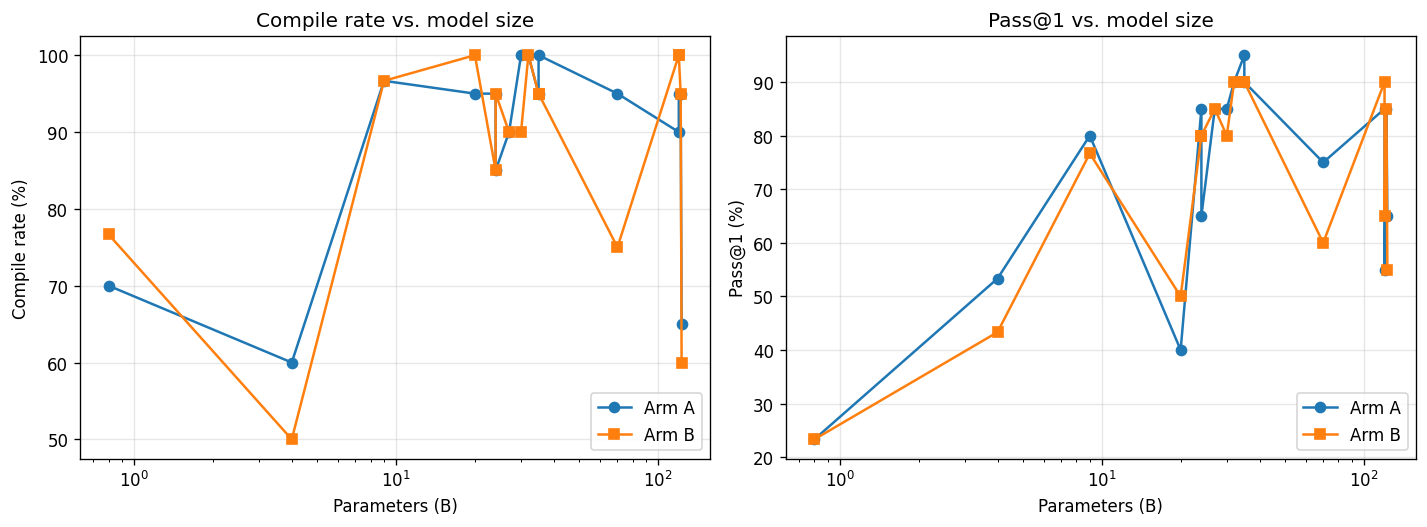
\includegraphics[width=\linewidth]{../results/week4/plots/blog_pass_compile_by_size.png}
    \caption{Compile rate and pass@1 vs. parameter count. Both arms saturate by $\sim$30B; the largest arm-wise gaps are at small scales.}
    \label{fig:passcompile}
\end{figure}

\subsection{H1 --- Is \armA\ faster than \armB?}

Short answer: no. Figure~\ref{fig:paired} shows paired median wall-clock per model. \armA\ is consistently $\geq$ \armB, sometimes by 2--3$\times$ at the larger models (e.g., \texttt{nemotron-3-super:120b}: \armA\ median 0.90\,s, \armB\ 0.86\,s; \armB\ total wall is an astonishing \textbf{21\,s for 20 problems with zero rollbacks}; \armA\ took 160\,s for the same problems). The LSP-blocking overhead on a per-boundary basis accumulates without producing actionable signal.

\begin{figure}[H]
    \centering
    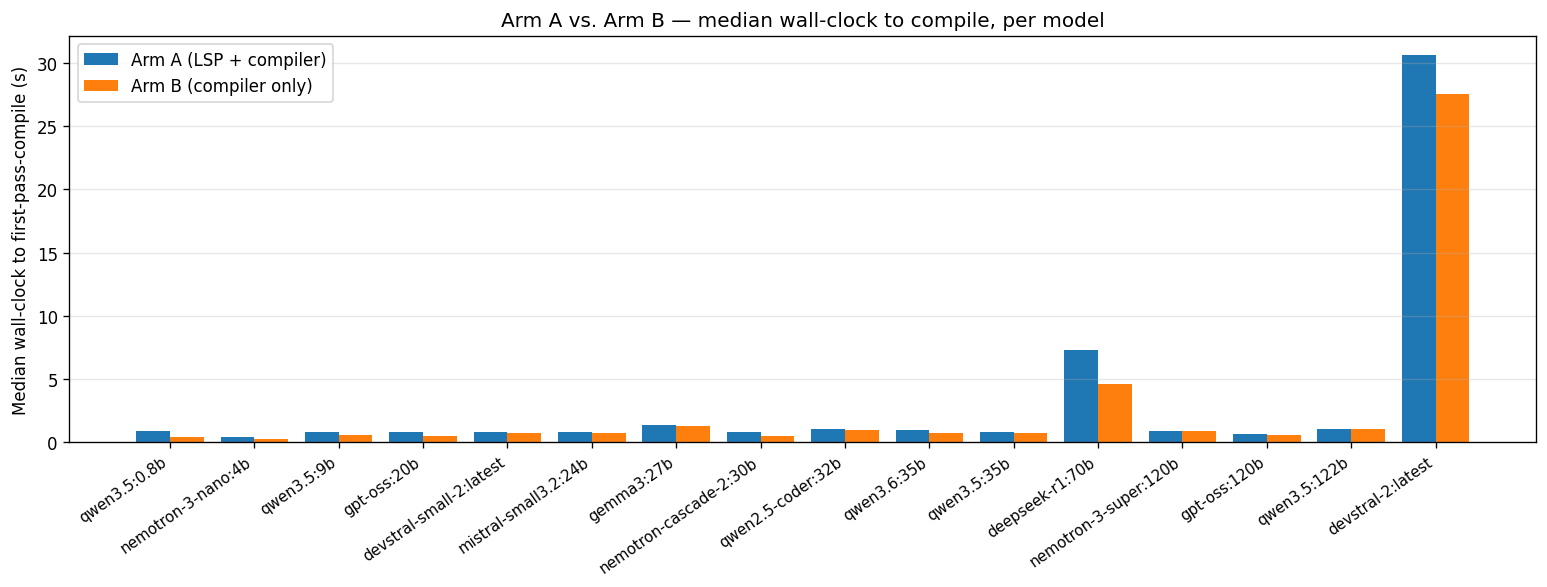
\includegraphics[width=\linewidth]{../results/week4/plots/blog_paired_wall.png}
    \caption{Per-model median wall-clock to first-pass-compile. Arm A consistently slower when both arms compile; the gap is largest at sizes where first-try success is already high (rollback machinery adds latency without helping).}
    \label{fig:paired}
\end{figure}

Wilcoxon signed-rank on paired wall-clock finds \armA\ significantly slower than \armB\ at several sizes (\texttt{nemotron-3-nano:4b} $p\!=\!0.0006$, \texttt{nemotron-cascade-2:30b} $p\!=\!0.002$, \texttt{nemotron-3-super:120b} $p\!=\!0.048$, \texttt{gpt-oss:20b} $p\!=\!0.014$). No size shows \armA\ significantly faster.

\subsection{H1(b) --- Does \armA\ use fewer compiler calls?}

Also no. Median compiler calls per problem is \textbf{1.0 for both arms at every model}. Why? The root cause turns out to be architectural (see Section~\ref{sec:architectural}): the LSP tier emits zero blocking classifications across the entire 15-model run. Every compiler call that would have fired in \armB\ fires identically in \armA. \armA\ can tie but cannot reduce compiler calls below \armB.

\subsection{H2 --- The partial scaling law}

Strongly supported on both arms. Figure~\ref{fig:rollback_scaling} shows rollback frequency collapsing from $\sim$5 per problem at 0.8B to near-zero at 30B+.

\begin{figure}[H]
    \centering
    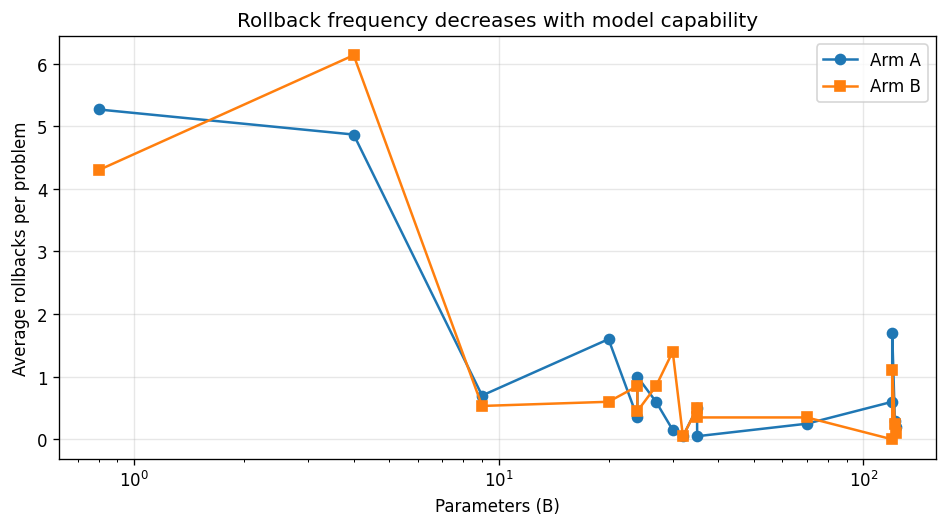
\includegraphics[width=0.78\linewidth]{../results/week4/plots/blog_rollback_scaling.png}
    \caption{Rollback frequency drops sharply with model size. Above 9B, most problems succeed on first try.}
    \label{fig:rollback_scaling}
\end{figure}

Spearman correlations across 15 sizes:

\begin{table}[H]
    \centering
    \caption{Scaling correlations (Spearman $\rho$). Both directions of the partial scaling law are statistically significant on both arms.}
    \begin{tabular}{lcc}
        \toprule
        \textbf{Correlation} & $\rho$ & $p$ \\
        \midrule
        \armA: params $\leftrightarrow$ compiler\_calls & $-0.608$ & $0.012$ \\
        \armA: params $\leftrightarrow$ wall-to-compile & $+0.513$ & $0.042$ \\
        \armB: params $\leftrightarrow$ compiler\_calls & $-0.682$ & $0.004$ \\
        \armB: params $\leftrightarrow$ wall-to-compile & $+0.681$ & $0.004$ \\
        \bottomrule
    \end{tabular}
    \label{tab:scaling}
\end{table}

Bigger models make fewer mistakes; bigger models take longer per token. Both directions hold with $p<0.05$ on both arms. This is the cleanest confirmation of the partial scaling law at this scale.

\subsection{H3 --- Coding-specialized saturation}

Confirmed. \texttt{qwen2.5-coder:32b}, \texttt{qwen3.5:35b}, and \texttt{qwen3.6:35b} all hit 100\% or near-100\% compile with $\leq 0.5$ avg rollbacks. Arm A and Arm B results are within 1 percentage point on all three, and \texttt{qwen3.6:35b} achieves the highest pass@1 in the entire evaluation at \textbf{95\%}. For these models, rollback as a mechanism has almost nothing to work with.

\subsection{Which arm wins per model?}

Figure~\ref{fig:winners} shows the per-model pass-rate delta (\armA\ $-$ \armB). Across 15 models: 5 favor \armA\ clearly, 5 are effectively tied, 5 favor \armB\ clearly. The split is roughly even and appears dominated by stochastic variance in 20-problem samples rather than a systematic function of model size.

\begin{figure}[H]
    \centering
    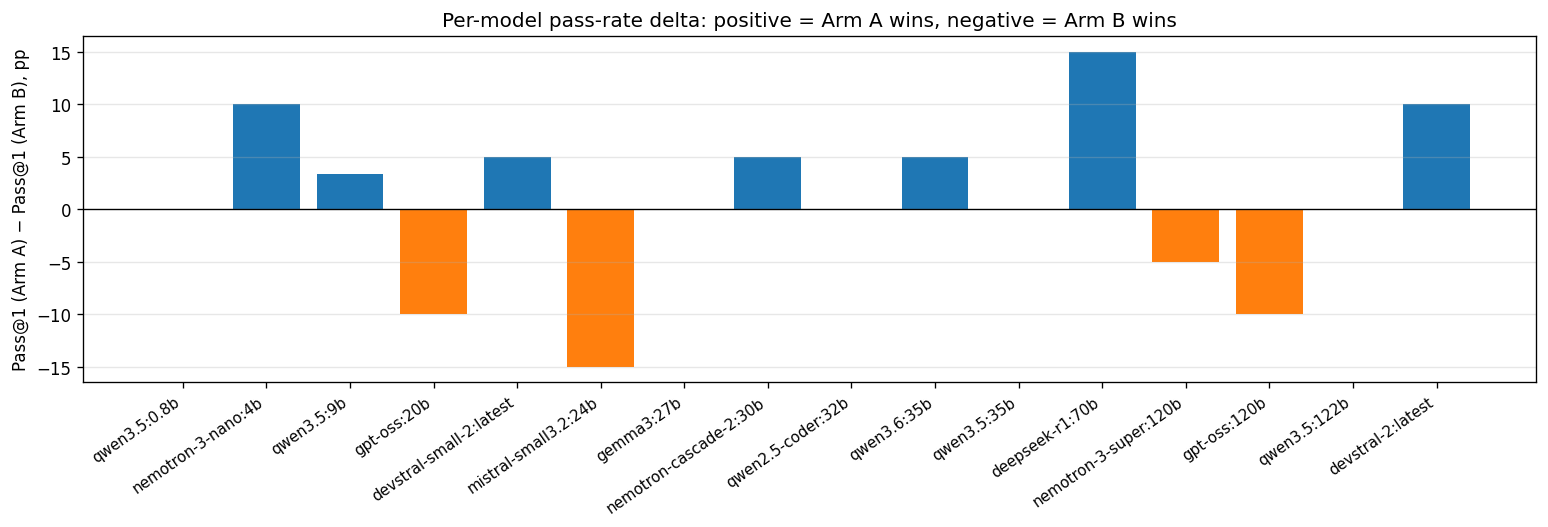
\includegraphics[width=\linewidth]{../results/week4/plots/blog_arm_winners.png}
    \caption{Per-model pass-rate delta (\armA\ $-$ \armB), sorted by parameter count. Positive bars = \armA\ wins; negative = \armB\ wins. No clear monotone pattern with size.}
    \label{fig:winners}
\end{figure}

One genuine surprise: \texttt{deepseek-r1:70b}, a reasoning model that emits \texttt{<think>$\ldots$</think>} blocks, produced the \emph{largest} arm-A margin (95\% vs. 75\% compile, 75\% vs. 60\% pass). This was entirely unexpected since the runner makes no allowance for thinking tokens --- they flow through as if they were Rust source. The model was also the only one producing borrow-checker errors (\texttt{E0382}, \texttt{E0505}) at any frequency; its reasoning apparently generates more complex code that exercises the borrow checker.

\subsection{Where does the time actually go?}

Figure~\ref{fig:profile} shows the wall-clock breakdown per category per (model, arm). Generation dominates everywhere (80--95\%). LSP-wait (the blocking component of \armA) is a small single-digit percentage but, critically, pays for nothing in our data.

\begin{figure}[H]
    \centering
    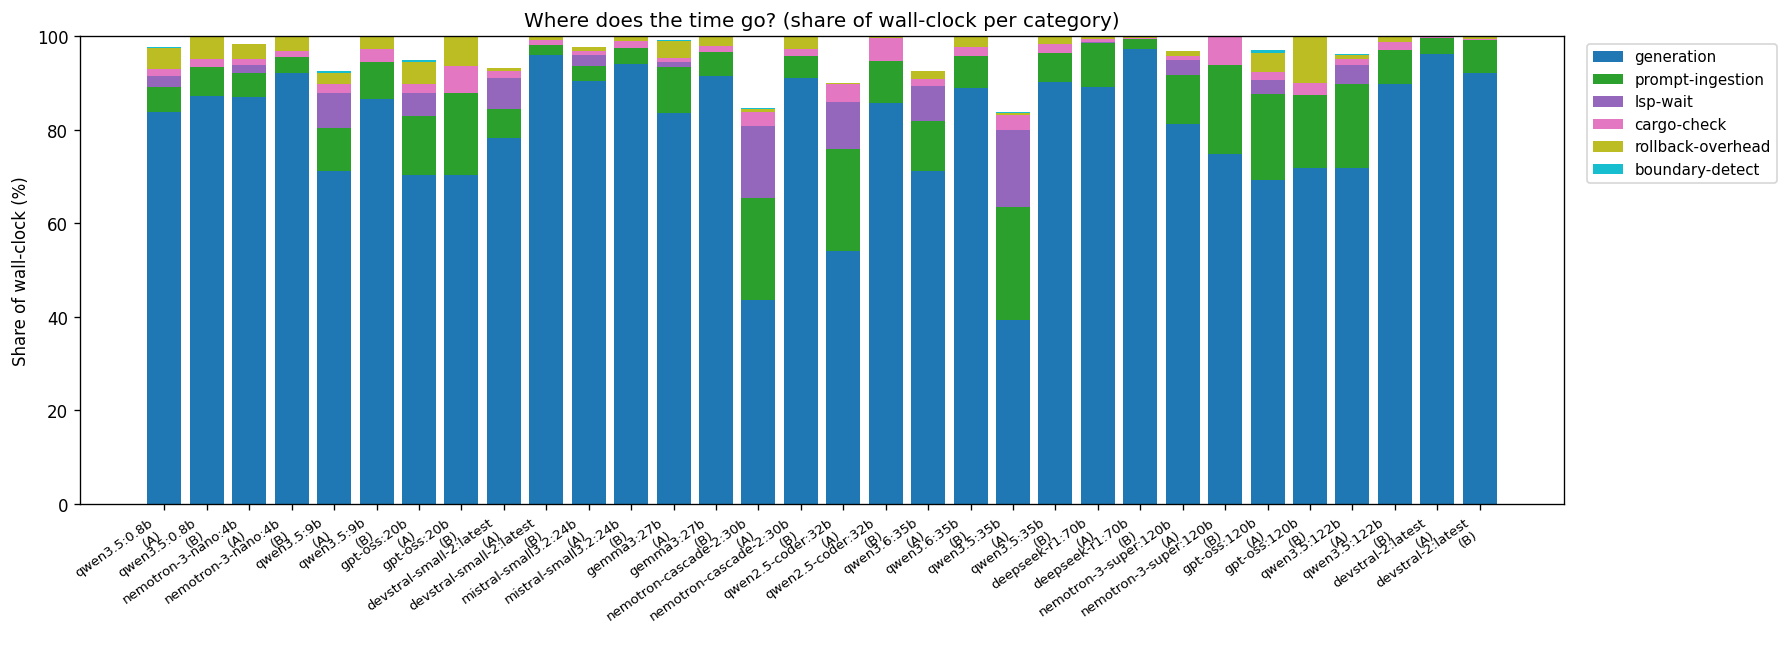
\includegraphics[width=\linewidth]{../results/week4/plots/blog_profile_share.png}
    \caption{Share of wall-clock per category, per (model, arm). Generation dominates. \armA's LSP overhead (\texttt{lsp-wait}, top-of-stack in blue band) visible but small; rollback-overhead on Ollama adds 3--5\%. Generation itself accounts for 80--95\% everywhere.}
    \label{fig:profile}
\end{figure}

\section{The Architectural Finding}
\label{sec:architectural}

The LSP tier of \armA\ fires zero blocking classifications across the entire evaluation. Concretely: across 15 models, 30 model-arm combinations, and over 2,000 classifier invocations, \textbf{the count of diagnostics classified as ``blocking'' is zero}. This is not a bug.

Here is what happens, traced through the classifier:

\begin{enumerate}
    \item During statement-by-statement generation, the enclosing function body is \emph{open} until the final closing brace. This is always the case during generation.
    \item The classifier's demotion rule downgrades \texttt{type-mismatch} (E0308) and \texttt{unresolved-reference} (E0425) to non-blocking whenever the function body is open --- necessary because these error codes fire on forward references the model will likely define later in the same function.
    \item Empirically, \texttt{type-mismatch} and \texttt{unresolved-reference} are the dominant native diagnostic codes rust-analyzer emits on partial Rust code. Other codes it catches (\texttt{unresolved-import}, syntax errors) are either rare or already treated as non-blocking.
\end{enumerate}

The intersection ``errors native diagnostics emit during partial generation'' $\cap$ ``errors the classifier considers blocking'' is approximately empty. The LSP tier is mechanically firing but producing no rollback-triggering signal. It is vestigial on this workload.

This is, in a sense, the most interesting finding of the week. The classifier rule is correct --- firing on every type-mismatch during generation would false-alarm constantly, as many type-mismatches resolve themselves once the next line is written. But the demotion rule and rust-analyzer's partial-code diagnostic coverage overlap almost exactly, leaving nothing for the tier to act on.

\subsection{How to fix it (Week 5 direction)}

Three candidate redesigns:

\begin{description}
    \item[Selective demotion.] Demote only \texttt{unresolved-reference} (the common forward-reference case), not \texttt{type-mismatch}. A type mismatch on a completed expression is usually real even if the rest of the function isn't written.
    \item[Cargo check at statement boundaries.] Replace native diagnostics with incremental \texttt{cargo check}. Has ground truth; no demotion needed. Cost: 500\,ms--2\,s per call, requiring careful batching.
    \item[Fully async LSP + async cargo check at function boundaries.] Don't block generation at all; fire cargo check in the background at each closed function and rollback only when it returns with a real error. Preserves the statement-boundary speculative generation but drops the mid-generation aborts.
\end{description}

\section{Conclusions}
\label{sec:conclusions}

\begin{itemize}
    \item \textbf{H1 falsified.} \armA\ is consistently slower than \armB\ at matched wall-clock budgets; it never wins on compiler-call count because its LSP tier produces no blocking signal.
    \item \textbf{H2 strongly supported.} Bigger models make fewer mistakes and take longer per token; both Spearman correlations are significant on both arms across 15 sizes.
    \item \textbf{H3 confirmed.} Coding-specialized models saturate to $\sim$100\% compile; rollback has nothing to contribute.
    \item \textbf{Architectural insight.} The null result is not ``rollback doesn't work'' --- it's ``the specific form of rollback feedback rust-analyzer's native diagnostics can provide is neutralized by the classifier demotion rule.''
\end{itemize}

The project's distinctive contribution --- external semantic verification with rollback --- runs directly into a design tension that MGD (completion-based, not diagnostic-based) and DSVD (internal probes, not external LSP) avoid for different reasons. Resolving the tension requires either selective demotion with clearer distinguishing rules, or a ground-truth verifier (cargo check) at the cost of latency.

Week 5 will migrate to HuggingFace \texttt{transformers} with token-level KV-cache truncation (eliminating the rollback-overhead cost), experiment with cargo-check-at-boundaries, and report on whether the redesigned LSP tier can actually contribute.

\subsection*{Reproducibility}

All code, raw per-problem profile JSONs, and the analysis notebook are at \texttt{./soundcode/eval/} and \texttt{./results/week4/}. The eval can be re-run with:
\begin{lstlisting}
uv run python -m soundcode.eval.experiment_week4 --arms A B --limit 20 --budget 60
uv run python -m soundcode.eval.analyze_week4 --plots
\end{lstlisting}

\end{document}
